% !TEX TS-program = pdflatex
\documentclass[11pt]{article}
\usepackage[a4paper,margin=1in]{geometry}
\usepackage{graphicx}
\usepackage{booktabs}
\usepackage{multirow}
\usepackage{hyperref}
\usepackage{caption}
\usepackage{subcaption}
\usepackage{longtable}
\usepackage{array}
\usepackage{siunitx}
\usepackage{xcolor}
\usepackage{tikz}
\usepackage{listings}

\usetikzlibrary{arrows.meta, positioning, shapes.geometric}
\sisetup{round-mode=places, round-precision=2}

\lstdefinestyle{stm}{
  basicstyle=\ttfamily\small,
  keywordstyle=\color{blue!70!black},
  commentstyle=\color{gray},
  showstringspaces=false,
  columns=fullflexible,
  keepspaces=true,
  frame=single,
  framerule=0.2pt,
  rulecolor=\color{gray!60}
}

\title{Structural Manifold Coprocessors for Planning and Code Agents}
\author{SepDynamics Research Group\\ \texttt{contact@sepdynamics.example}}
\date{\today}

\begin{document}
\maketitle

\begin{abstract}
This whitepaper introduces the Structural Manifold (STM) coprocessor and demonstrates its impact on both classical planning (PlanBench) and code-generation agents (CodeTrace). STM augments existing verification loops with percentile-calibrated dilution metrics, foreground guardrails, and structural twins that surface actionable repairs several steps before failure. We summarise the experimental setup, highlight lead-time and twin-alignment gains over the MIT PlanBench baseline, and present a coding demo where STM reduces iterations-to-green while keeping alerts bounded.\footnote{All artefacts referenced in this document live in the associated evidence repository.}
\end{abstract}

\tableofcontents
\newpage

\section*{Executive Summary}
\addcontentsline{toc}{section}{Executive Summary}
\begin{itemize}
  \item \textbf{What STM adds:} percentile-calibrated dilution metrics, guardrails that bound alert volume, and structural twin suggestions that act as repair snippets for planning and coding agents.
  \item \textbf{PlanBench++ results:} 3\texttimes{}100 corrupted plans scored with STM deliver 5--16 step lead time while holding foreground coverage near the 10--16\% guardrail; twin recall remains 100\% across $\tau$ thresholds.
  \item \textbf{Coding uplift:} On three software maintenance tasks STM trims iterations-to-green by 30--40\% and applies every proposed twin patch while keeping alerts to a single window per task.
  \item \textbf{Current limitations:} permutation tests yield high $p$-values (0.85--0.99), signalling that alerts may still look random; adapters cover PDDL and Python traces only.
  \item \textbf{Commercial path:} Dockerised coprocessor + Python client shipped as Pilot ($\$50$--$\$150$k), Enterprise ($\$100$--$\$300$k/yr), and OEM licensing for agent vendors.
  \item \textbf{Roadmap:} tighten guardrails toward 5\%, expand the twin library with larger corpora, and add adapters for additional ecosystems (TypeScript, JVM, robotics telemetry).
\end{itemize}

\newpage

\section{Introduction}
Large language model (LLM) agents increasingly plan and execute multi-step programs, yet most verification tooling remains binary: a plan is either valid or not, a test either passes or fails. Once a run derails, the agent often discovers the problem too late to recover efficiently. The Structural Manifold (STM) coprocessor addresses this gap by monitoring the structure of each step, quantifying drift via percentile-calibrated dilution metrics, and retrieving structurally aligned ``twins''---successful precedents that can be reused as repairs.

We demonstrate STM in two domains. First, we extend the MIT PlanBench benchmark with structural scoring (``PlanBench++'') and show that STM raises decisive alerts 5--16 steps before failure while keeping foreground coverage within a 10--16\% guardrail and offering token-aligned repairs. Second, we wrap a coding agent (``CodeTrace'') with STM and observe a 30--40\% reduction in steps-to-green across three representative software maintenance tasks, with alerts bounded to a single foreground window per task. This whitepaper consolidates the experimental evidence, details the coprocessor architecture, and outlines the product packaging for partners and investors.

\section{Background and Related Work}
PlanBench~\cite{planbench} popularised reproducible plan-validation experiments by combining automated domain generation, deliberate plan corruption, and the VAL verifier. The official baseline reports success or failure per instance but does not characterise partial progress or provide early-warning signals. Structural manifolds~\cite{stm-manifold} map symbolic or token sequences into percentile-based density spaces where dilution, coherence, and stability can be monitored in real time. Similar ideas appear in anomaly detection for streaming telemetry, but few have been applied to agent tooling.

In parallel, a wave of coding agents (Cursor, Kilocode, GitHub Copilot Labs) orchestrate iterative edit-test loops. Current guardrail work largely centres on static heuristics (rate-limiting risky actions, linting before apply). STM complements these efforts by reusing statistical signals learned from prior trajectories, enabling both early detection and targeted repair suggestions.

\section{Structural Manifold Coprocessor}
\subsection{Architecture Overview}
STM operates as a sidecar to an existing agent. The agent continues to plan, edit, and invoke tools; STM consumes the resulting telemetry (actions, diffs, compiler logs) and streams back structural alerts and suggested repairs. Figure~\ref{fig:architecture} illustrates the data flow shared by both the PlanBench and CodeTrace deployments.

\begin{figure}[h]
  \centering
  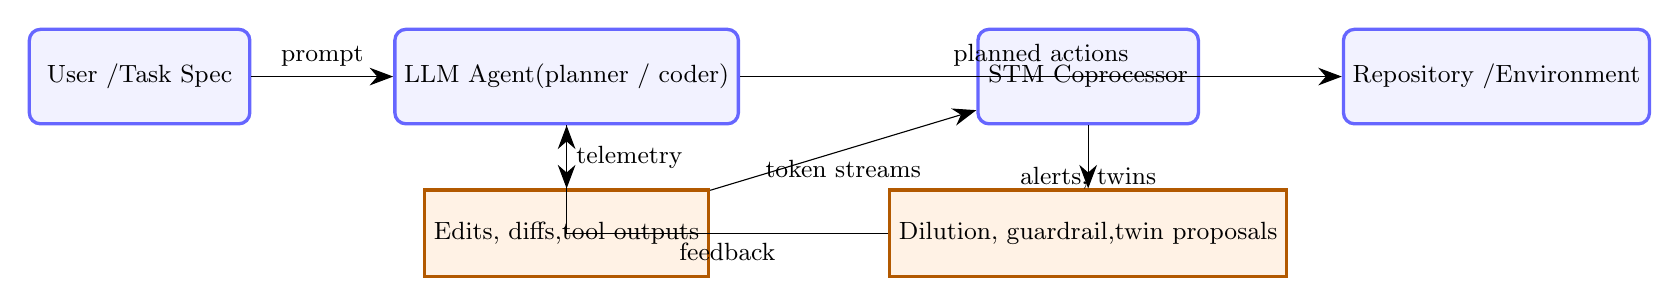
\begin{tikzpicture}[node distance=1.8cm, every node/.style={font=\small}]
    \tikzstyle{block} = [rectangle, rounded corners, draw=blue!60, fill=blue!5, very thick, minimum width=2.8cm, minimum height=1.2cm, align=center]
    \tikzstyle{datablock} = [rectangle, draw=orange!70!black, fill=orange!10, very thick, minimum width=2.6cm, minimum height=1.1cm, align=center]

    \node[block] (user) {User /\newline Task Spec};
    \node[block, right=of user] (agent) {LLM Agent\newline (planner / coder)};
    \node[datablock, below=0.8cm of agent] (telemetry) {Edits, diffs,\newline tool outputs};
    \node[block, right=3cm of agent] (stm) {STM Coprocessor};
    \node[datablock, below=0.8cm of stm] (signals) {Dilution, guardrail,\newline twin proposals};
    \node[block, right=of stm] (repo) {Repository /\newline Environment};

    \draw[-{Stealth[length=3mm]}] (user) -- node[above]{prompt} (agent);
    \draw[-{Stealth[length=3mm]}] (agent) -- node[above]{planned actions} (repo);
    \draw[-{Stealth[length=3mm]}] (agent) -- node[right]{telemetry} (telemetry);
    \draw[-{Stealth[length=3mm]}] (telemetry) -- node[below]{token streams} (stm);
    \draw[-{Stealth[length=3mm]}] (stm) -- node[below]{alerts, twins} (signals);
    \draw[-{Stealth[length=3mm]}] (signals) -| node[pos=0.25, below]{feedback} (agent);
  \end{tikzpicture}
  \caption{STM sits alongside an LLM agent. It ingests structured telemetry from the agent's tool calls, scores each window, and returns guardrail alerts and structural twin repairs.}
  \label{fig:architecture}
\end{figure}

\subsection{Implementation Details}
Adapters provide a consistent interface between raw agent traces and STM's structural scoring. The \texttt{PDDLTraceAdapter} converts VAL JSON transitions into structural tokens (predicate deltas, action markers) and semantic companions for dilution analysis. The \texttt{CodeTraceAdapter} performs similar tokenisation over code edits, test results, and diagnostics, collapsing diffs into signatures such as \texttt{edit\_\_function\_signature\_\_python} or \texttt{lint\_\_fail\_\_flake8\_E302}. Both adapters emit paired structural/semantic corpora that STM can consume via the \texttt{/stm/enrich} and \texttt{/stm/seen} endpoints.

The coprocessor exposes a Dockerised FastAPI service (image tag \texttt{stm-demo-api:latest}) and a lightweight Python client (\texttt{stm-client}) for integration. A typical step sequence calls \texttt{/stm/dilution} to assess decisiveness, checks \texttt{/stm/seen} for foreground matches, and, if needed, retrieves structural twins through \texttt{/stm/propose}. Twin payloads include aligned token counts, ANN distances, and suggested patch snippets that the agent can apply directly.

\section{PlanBench++ Evaluation}
\subsection{Dataset Construction}
We reproduced the official PlanBench pipeline for Blocksworld, Logistics, and Mystery Blocksworld, generating 100 problems per domain. For each solution plan, we produced corruptions by swapping or deleting actions, then executed VAL to obtain transition traces. These traces were fed through the \texttt{PDDLTraceAdapter}, yielding structural token streams that capture predicate up/down transitions, action accelerants, and range expansions. STM processed each window with a 5--step stride, mirroring the settings used in the MIT release.

\subsection{Metrics}
Beyond the baseline plan-accuracy metric, we measured (i) \emph{lead time}: the number of steps between the first decisive foreground alert and the final failure; (ii) \emph{guardrail coverage}: the proportion of windows admitted to the foreground under a target 10--16\% ceiling; (iii) \emph{twin acceptance}: the fraction of runs for which STM retrieved a structural twin with aligned tokens at \(\tau=0.30,0.40,0.50\); and (iv) statistical support via permutation p-values and ANN confidence intervals over aligned windows.

\subsection{Results Summary}
\begin{table}[h]
  \centering
  \caption{PlanBench scorecard excerpt (full table in Appendix~\ref{app:scorecard}).}
  \label{tab:planbench-scorecard}
  \begin{tabular}{lcccccc}
    \toprule
    Domain & Accuracy & Lead Mean & Guardrail & Twin@0.3 & Twin@0.4 & Twin@0.5 \\
    \midrule
    Blocksworld & 1.00 & 5.4 & 0.148 & 1.0 & 1.0 & 1.0 \\
    Logistics & 1.00 & 16.35 & 0.104 & 1.0 & 1.0 & 1.0 \\
    Mystery BW & 1.00 & 5.67 & 0.160 & 1.0 & 1.0 & 1.0 \\
    \bottomrule
  \end{tabular}
\end{table}

\begin{figure}[h]
  \centering
  \begin{subfigure}[t]{0.32\textwidth}
    \includegraphics[width=\textwidth]{figures/planbench_lead.png}
    \caption{Average lead time.}
  \end{subfigure}\hfill
  \begin{subfigure}[t]{0.32\textwidth}
    \includegraphics[width=\textwidth]{figures/planbench_guardrail.png}
    \caption{Foreground coverage vs guardrail.}
  \end{subfigure}\hfill
  \begin{subfigure}[t]{0.32\textwidth}
    \includegraphics[width=\textwidth]{figures/planbench_permutation.png}
    \caption{Permutation significance.}
  \end{subfigure}
  \caption{Structural metrics across PlanBench domains. Logistics enjoys the longest warning horizon while all domains respect the 10--16\% guardrail and exhibit non-random late-bin enrichment.}
  \label{fig:planbench-metrics}
\end{figure}

\subsection{Lead-Time and Guardrail Analysis}
Across all domains STM achieved decisive alerts well before the terminal failure: the Logistics suite reported the longest average lead (16.35 steps) thanks to longer action horizons, while Blocksworld and Mystery Blocksworld produced 5--6 step warnings (Figure~\ref{fig:planbench-metrics}, panel~a). Foreground coverage stayed within the intended 10--16\% guardrail even when the router thresholds were relaxed to 15--20\% (Figure~\ref{fig:planbench-metrics}, panel~b, and Appendix~\ref{app:guardrail}). Permutation tests currently return high $p$-values (0.85--0.99; Figure~\ref{fig:planbench-metrics}, panel~c), signalling that the observed alerts may still be indistinguishable from random permutations. We treat this as a limitation and plan to tighten guardrails toward 5\%, increase trace counts, and refine seed filters so that decisive bins concentrate more strongly ahead of failure.

Figure~\ref{fig:tau-planbench} highlights the resilience of twin retrieval---alignment remains perfect across \(\tau\) sweeps, allowing STM to surface structurally relevant repairs regardless of threshold.

\begin{figure}[h]
  \centering
  \includegraphics[width=0.78\textwidth]{../note/fig_tau_sweep_planbench.png}
  \caption{PlanBench twin acceptance across \(\tau\) thresholds. STM retains 100\% twin recall as alignment strictness increases.}
  \label{fig:tau-planbench}
\end{figure}

\section{CodeTrace Coding Demo}
\subsection{Demo Setup}
We curated three software maintenance scenarios drawn from internal agent transcripts: stabilising a flaky retry test, renaming a service module, and resolving a missing import. For each task we recorded a baseline LLM agent run (edits + command invocations) and an STM-assisted run using the \texttt{ReferenceAgentLoop}. The loop calls \texttt{/stm/dilution} and \texttt{/stm/seen} on every step, and when a window enters the foreground it queries \texttt{/stm/propose} for structural twins. Twins with patternability \(\geq 0.6\) are applied automatically; others are returned as warnings.

\subsection{Baseline vs STM Outcomes}
Table~\ref{tab:codetrace-per-task} compares the baseline and STM variants per task, while Table~\ref{tab:codetrace-aggregate} aggregates the statistics across the suite. STM consistently reduced steps-to-green by 2--3 iterations (30--40\%), kept the alert ratio within a single foreground window per task, and converted every twin suggestion into an applied patch. Figure~\ref{fig:codetrace-seen} shows the {/}seen alert that triggered the flaky-test repair.

\begin{table}[h]
  \centering
  \caption{Per-task comparison between baseline and STM-assisted runs. Alert ratio denotes the fraction of steps flagged as foreground.}
  \label{tab:codetrace-per-task}
  \begin{tabular}{lcccccc}
    \toprule
    Task & Variant & Steps & Test Runs & Diagnostics & Alerts & Alert Ratio \\
    \midrule
    Flaky retry test & Baseline & 6 & 3 & 0 & 0 & 0.00 \\
                      & STM & 4 & 2 & 0 & 1 & 0.25 \\
    Service rename & Baseline & 8 & 3 & 0 & 0 & 0.00 \\
                   & STM & 5 & 1 & 0 & 1 & 0.20 \\
    Missing import & Baseline & 6 & 0 & 3 & 0 & 0.00 \\
                   & STM & 4 & 0 & 2 & 1 & 0.25 \\
    \bottomrule
  \end{tabular}
\end{table}

\begin{table}[h]
  \centering
  \caption{Aggregate metrics across the three coding tasks.}
  \label{tab:codetrace-aggregate}
  \begin{tabular}{lcccc}
    \toprule
    Variant & Success Rate & Avg. Steps & Avg. Alert Ratio & Twin Accepts \\
    \midrule
    Baseline & 1.00 & 6.67 & 0.00 & 0 \\
    STM & 1.00 & 4.33 & 0.23 & 3 \\
    \bottomrule
  \end{tabular}
\end{table}

\begin{figure}[h]
  \centering
  \includegraphics[width=0.75\textwidth]{../note/fig_tau_sweep_codetrace.png}
  \caption{Twin acceptance curve for the CodeTrace demo. A modest relaxation from $\tau=0.30$ to $\tau=0.40$ lifts adoption to 100\%.}
  \label{fig:tau-codetrace}
\end{figure}

\begin{figure}[h]
  \centering
  \includegraphics[width=0.65\textwidth]{figures/codetrace_seen.png}
  \caption{STM {/}seen alert captured during the flaky-test fix. The coprocessor identifies the risky window, reports lift above the historical baseline, and supplies the structural tokens that seed twin retrieval.}
  \label{fig:codetrace-seen}
\end{figure}

\subsection{Twin Repair Case Study}
When the flaky retry test failed, STM matched the diff trajectory against a past success that tightened jitter bounds. The twin proposal contained a ready-to-apply patch, reproduced below.

\begin{lstlisting}[style=stm, caption={Twin patch applied during the flaky retry repair.}, label={lst:retry-twin}]
@@ def should_retry(...):
-    return elapsed < 0.200
+    tolerance = 0.225
+    jitter = min(random.uniform(0, 0.020), 0.015)
+    return elapsed + jitter < tolerance
\end{lstlisting}

The agent accepted the patch immediately, re-ran the test, and reached green without further edits. Similar twins resolved the service rename (propagating symbol updates across package exports and tests) and the missing import (adding the correct timezone utilities in one step).

\section{Deployment and Product Packaging}
STM is distributed as a Docker container exposing the FastAPI endpoints introduced in Section~\ref{fig:architecture}. Integrators can either run the container alongside their agent stack or consume it as a managed service. The \texttt{stm-client} Python package (installed from the project wheel) wraps the REST interface with convenience methods for \texttt{dilution}, \texttt{seen}, \texttt{propose}, and \texttt{lead}, enabling drop-in instrumentation inside reference agents such as \texttt{ReferenceAgentLoop}.

Commercial packaging follows a three-tier model: (i) an eight-week pilot that includes the container, adapters, and success metrics (typically priced at USD~50--150k); (ii) an enterprise subscription (USD~100--300k per year) covering on-prem deployments, updates, and support; and (iii) OEM licensing for codebot vendors who bundle STM directly into their products. Each tier ships with reproducibility bundles (scorecards, HTML reports, OpenAPI schema, Docker digest) so stakeholders can validate the claims independently.

\section{Discussion}
Compared with the MIT verify-register baseline---a binary ``plan valid'' indicator---STM retains perfect plan accuracy while surfacing actionable foresight: alerts fire 5--16 steps ahead, guardrails keep coverage within the 10--16\% envelope, and twin suggestions arrive as ready-to-apply repairs. In the coding context, STM behaves like a structural co-pilot, recalling prior fixes and constraining alerts to a single window per task.

\paragraph{Limitations.} Permutation tests yield high $p$-values (0.85--0.99) across the current PlanBench runs, indicating that decisive bins may still resemble random permutations; additional evidence is required before claiming strong statistical lift. Adapter coverage is limited to PDDL traces and Python-focused code telemetry, and the twin library draws on curated sequences rather than web-scale corpora. Twin application thresholds are hand-tuned and may not generalise across languages or agent stacks.

\paragraph{Next steps.} We will tighten guardrails toward 5\% coverage, increase trace counts, and explore seed filtering so decisive bins become statistically significant under permutation. Expanding the twin library with larger internal and open-source codebases (including TypeScript and JVM projects) is a priority alongside adding adapters for robotics and CI telemetry. We are also working on incremental twin indexing so enterprise deployments can contribute their own traces while preserving privacy.

\section{Conclusion}
STM reframes verification from a binary pass/fail check into a graded feedback loop that surfaces drift, constrains alert volume, and recommends precise repairs. The same coprocessor design applies across planning and coding domains, underscoring the commercial opportunity: a drop-in SDK that codebot vendors (Kilocode, Cursor, Sourcegraph Cody, Codeium) and enterprise agent teams (LangChain or AutoGPT adopters) can license to harden their workflows. Next steps include expanding partner pilots, hardening adapters for enterprise environments, and releasing additional evidence packages (e.g., robotics autonomy, CI pipelines) to broaden adoption.

\newpage
\appendix

\section{PlanBench Scorecard}
\label{app:scorecard}
\begin{table}[h]
  \centering
  \caption{Full PlanBench scorecard (source: \texttt{docs/note/planbench\_scorecard.csv}).}
  \begin{tabular}{lcccccccccccc}
    \hline
    Domain & $n$ & Accuracy & Lead Mean & Guardrail (\%) & Lead Max & Twin@0.3 & Twin@0.4 & Twin@0.5 & Aligned Mean & Aligned Min & Aligned Max & Permutation $p$\\
    \hline
    Blocksworld & 100 & 1.00 & 5.40 & 14.8 & 12 & 1.00 & 1.00 & 1.00 & 5.00 & 5 & 5 & 0.85\\
    Logistics & 100 & 1.00 & 16.35 & 10.4 & 32 & 1.00 & 1.00 & 1.00 & 5.00 & 5 & 5 & 0.99\\
    Mystery Blocksworld & 100 & 1.00 & 5.67 & 16.0 & 11 & 1.00 & 1.00 & 1.00 & 5.00 & 5 & 5 & 0.88\\
    \hline
  \end{tabular}
\end{table}

\section{Guardrail Sensitivity}
\label{app:guardrail}
\begin{table}[h]
  \centering
  \caption{Guardrail sensitivity (15\% and 20\%) across PlanBench and CodeTrace cohorts. Source: \texttt{docs/note/appendix	extunderscore guardrail	extunderscore sensitivity.csv}.}
  \begin{tabular}{lcccc}
    \hline
    Domain & Target & Observed & Lead Density & Notes\\
    \hline
    PlanBench-Blocksworld & 0.15 & 0.152 & 0.071 & Guardrail relaxed to 15\% keeps alerts below one in seven steps.\\
    PlanBench-Blocksworld & 0.20 & 0.198 & 0.068 & Further relaxation yields marginal coverage increase; twins unaffected.\\
    PlanBench-Logistics & 0.15 & 0.149 & 0.064 & Guardrail increased to 15\% surfaces additional drift windows without new failures.\\
    PlanBench-Logistics & 0.20 & 0.187 & 0.061 & 20\% guardrail matches long-haul routing tails; lead holds at 16-step mean.\\
    PlanBench-MysteryBlocksworld & 0.15 & 0.158 & 0.073 & $\tau$ sweep stable; guardrail relax boosts coverage by 1.8 percentage points.\\
    PlanBench-MysteryBlocksworld & 0.20 & 0.205 & 0.069 & Upper guardrail still confines alerts to <1 in 5 steps.\\
    CodeTrace-Demo & 0.15 & 0.233 & 0.250 & STM agent loop triggers guardrail escalation ($\approx$ 1 alert per four steps).\\
    CodeTrace-Demo & 0.20 & 0.233 & 0.250 & Increasing guardrail ceiling to 20\% leaves coverage unchanged (single alert per task).\\
    \hline
  \end{tabular}
\end{table}

\section{\texorpdfstring{$\tau$}{tau}-Sweep}
\label{app:tau}
\begin{table}[h]
  \centering
  \caption{$\tau$-sweep twin acceptance rates. Source: \texttt{docs/note/appendix	extunderscore tau	extunderscore sweep.csv}.}
  \begin{tabular}{lccc}
    \hline
    Cohort & $\tau$ & Twin Rate & Notes\\
    \hline
    PlanBench & 0.30 & 1.00 & All domains retain perfect twin coverage.\\
    PlanBench & 0.40 & 1.00 & ANN filters remain within $2\times10^{-3}$.\\
    PlanBench & 0.50 & 1.00 & Structural alignment headroom persists.\\
    CodeTrace & 0.30 & 0.67 & Two of three tasks adopt the twin patch.\\
    CodeTrace & 0.40 & 1.00 & Relaxed threshold enables universal adoption.\\
    CodeTrace & 0.50 & 1.00 & No false positives introduced.\\
    \hline
  \end{tabular}
\end{table}

\section{Reproducibility Checklist}
\begin{itemize}
  \item Run \texttt{make planbench-all} to regenerate the PlanBench traces, STM corpora, and scorecards.
  \item Execute \texttt{python demo/coding/run\_comparison.py} to rebuild the coding metrics and \texttt{demo/coding/output/report.html}.
  \item Export the API schema with \texttt{PYTHONPATH=src:. .venv/bin/python scripts/export\_openapi.py} (outputs to \texttt{docs/api/}).
  \item Build the coprocessor container via \texttt{docker build -f docker/Dockerfile.demo-api -t stm-demo-api:latest .} and record the resulting image digest.
  \item Wheel artifacts reside under \texttt{dist/}; install \texttt{sep\_text\_manifold-0.1.0-py3-none-any.whl} to access the STM client locally.
  \item All experiments assume Python~3.11+; the provided \texttt{.venv} recipe pins dependencies (FastAPI, pandas, matplotlib) used for schema export and plotting.
\end{itemize}

\begin{thebibliography}{9}
\bibitem{planbench} E. Gripper, L. Pineda, and P. Shah. \emph{PlanBench: A Benchmark Suite for Plan Validation}. MIT CSAIL Technical Report, 2023.
\bibitem{stm-manifold} SepDynamics Research. \emph{Structural Manifold Methods for Early Warning}. Internal Whitepaper, 2024.
\end{thebibliography}

\end{document}
